\chapter{Background and Related Work}
\label{chap:background}

This chapter surveys various concepts used in the thesis, including an introduction to automatic summarization, methods for evaluating summaries, as well as studies relating to Twitter data and tweet generation.


\section{Summarization}

Text summarization is the task of condensing an original text document or documents while retaining as much of the important information as possible \citep{mani-2001}. In addition, the summary must also satisfy goals related to the quality of the generated text, such as readability and coherence. The two main approaches for automatic text summarization are \textit{extractive} and \textit{abstractive} summarization. 

Extractive summarization uses the technique of choosing the important parts of the text and rearranging them to generate summaries. \cite{nenkova2012survey} describe the components in extractive summarization techniques as 
\begin{inparaenum}[1)]
\item{building an internal representation of the important parts of the text,}
\item{ranking these in the order of importance or time or other relevant metric based on context, and then }
\item{selecting a suitable list of these sentences to form the summary.}
\end{inparaenum}

 This selection of important parts of the source can be done at various levels, such as phrases, sentences, or paragraphs \citep{nenkova2012survey, hahn2000challenges}. In phrase-level summarization, smoothing techniques may be used to generate readable texts, since stitching together phrases from the source will lack coherence. In contrast to phrase-level summarization, sentence-level summarization techniques tend to be inherently more grammatically correct since sentences are directly picked out. However, sentence compression techniques can also be used to reduce the size of the summaries in sentence-level summarization \citep{knight2002summarization}. Even after using smoothing techniques to generate readable text, extractive summaries tend to be incoherent and hard to read \citep{liu2009extractive}. It should be noted that since we are dealing with the summaries being used as tweets, and since tweets are only 140 characters long, we will mostly be dealing with word-level or n-gram-level summarization. 


% \begin{figure}[!htbp]
% \centering
% 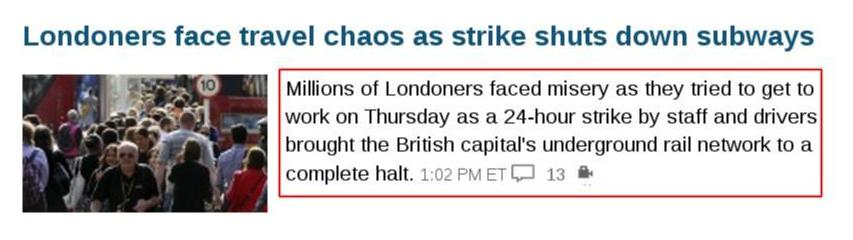
\includegraphics[width=\textwidth, height=4.5cm]{extractive}
% \caption{Example of extractive summarization.}
% \label{fig:extractive}
% \end{figure}


The second approach is that of abstractive summarization. This is a summarization approach that aims to keep the content or meaning of the input source the same while condensing the text or generalizing it, and involves text generation for generating the summary. As a rule, abstractive summarization requires world knowledge and is a much more difficult problem to solve. As a result, current summarization techniques concentrate on improving results from extractive summarization \citep{nenkova2012survey}. 

\begin{figure}[!t]
\centering
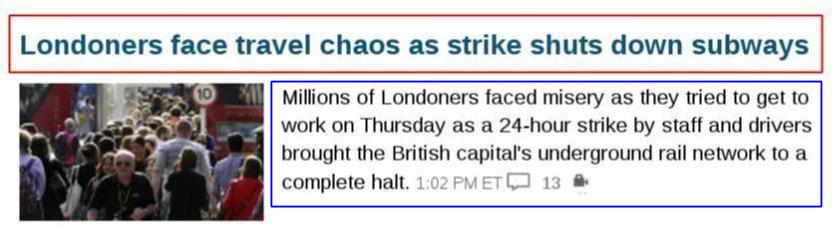
\includegraphics[width=\textwidth, height=4.5cm]{example_summarization}
\caption{Examples of extractive and abstractive summarization.}
\label{fig:examples}
\end{figure}

\figref{fig:examples} shows examples of both an extractive and abstractive summary in the form of a newspaper article thumbnail. The blue box outlines a few sentences from the article that have been picked to give a brief description. This acts as the extractive summary. The red box outlines the title of the article, which is an abstractive summary of the article; it is a generalization of the events described, carefully omitting details yet leaving the overall meaning of the event untouched.

% \figref{fig:extractive} shows an example of extractive summarization where a couple of sentences from the article have been picked to show in the the thumbnail for an article.

% \figref{fig:abstractive} shows the same thumbnail for a news article. However, the title of the article is an abstractive summary that is a generalization of the events described, carefully omitting details yet leaving the overall meaning of the event untouched.

% \begin{figure}[!htbp]
% \centering
% 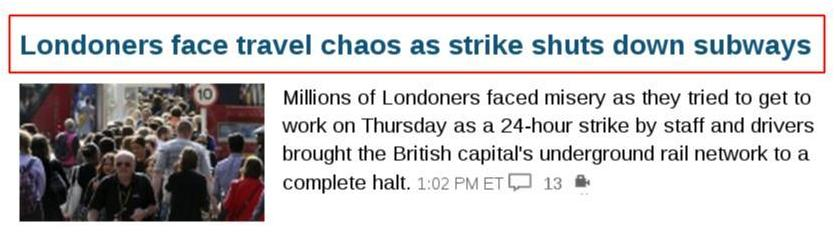
\includegraphics[width=\textwidth, height=4.5cm]{abstractive}
% \caption{Example of abstractive summarization.}
% \label{fig:abstractive}
% \end{figure}


Although extractive summarization has been predominant, there have been studies on its limitations. \cite{he2000comparing} compared user preferences for various mechanisms of browsing content from an audio-visual presentation. They demonstrated that the most preferred method of summarization was highlights and notes provided by the author, rather than transcripts or slides from the presentation, which can be viewed as the full source text and the compressed pointers for the presentation respectively. \cite{conroy2006topic} investigated the issue of limits of extraction by using an oracle ROUGE score based on a probabilistic model of unigrams that might appear in the gold standard summaries and exploit this to create a new method of summarization that uses maximum likelihood estimation.
% The oracle score is based on the maximum likelihood probability of words occurring in model summaries and is in turn used to generate summaries that perform better than any extracted and also human-generated summaries. 


\subsection{ROUGE: Evaluation Measure for Text Summarization}

ROUGE is an evaluation measure popularly used for evaluating the quality of summaries \citep{lin-2004}. It measures the quality of a summary by comparing the output of the system being tested against a set of gold standard summaries by word or n-gram overlap. The intuition is that if the generated summary has enough in common with a set of human-written summaries, then it can be judged as a good summary. The different types of comparisons calculated are the unigram, bigram, trigram and least common subsequence (ROUGE-1,2,3 and L respectively). A set of gold standard summaries are used to account for the fact that summary writers do not agree on the contents of the summary. 

\begin{equation}
\textit{ROUGE-n} = \frac{\sum\limits_{S \in \{Reference Summaries\}} \sum\limits_{gram_n \in S} Count_{match}(gram_n)}{\sum\limits_{S \in \{Reference Summaries\}} \sum\limits_{gram_n \in S} Count(gram_n)}
\end{equation}

The equation as described by \cite{lin2004looking} shows the calculation of the ROUGE-N score, where $n$ is the length of the n-gram, and $Count_{match}$ is the count of the matched n-grams in the summary and the reference summaries.

The use of multiple gold standard summaries gives rise to a subjective evaluation metric where the quality of the evaluation is dependent on the quality and number of the gold standard summaries. ROUGE also does not take into account whether the summary is fluent or coherent. However, ROUGE is useful for the evaluation of summarization methods for overall content retention from the original text. This is possible due to the use of n-gram co-occurrence statistics used by ROUGE.
% \section{Stylistics}
%\change{remove this and put it in the formality part}
% Stylistics is referred to the characteristics of text that can be extracted from it that do not relate to the meaning of the text. Common examples of these include textual statistics such as length of sentences and words, parts of speech, function words etc. and finds applications in authorship attribution, semantic analysis, personality typing and so on. Studies on building lexicons for formality have been conducted and are discussed further later \chapref{chap:analysis}.

\section{Studies Based on Twitter Data}

\subsection{Twitter Data and Summarization}

In this section, we discuss studies that use Twitter data as the source to study the summarization concepts discussed above.
% and other concepts which we consider in our user studies, such as classifying tweets based on who it was generated by, and sentiment analysis of tweets. 

The following studies focus on using summarization in relation to Twitter data. \cite{o2010tweetmotif} use topic summarization for a given search for better browsing. \cite{chakrabarti2011event} generate an event summary by learning about the event using a Hidden Markov Model over the tweets describing it. \cite{wang2014socially} generate a coherent event summary by treating summarization as an optimization problem for topic cohesion. \cite{inouye2011comparing} compare multiple summarization techniques to generate a summary of multi-post blogs on Twitter. \cite{wei2014utilizing} use tweets to help in generating better summaries of news articles.

% detailed analysis of this paper
As described in \chapref{chap:intro}, we analyze tweet generation using measures inspired by extractive summarization evaluation. \cite{lloret2013towards} compared the different text summarization techniques for tweet generation. Summarization systems were used to generate sentences which could then be taken to be tweets by summarizing documents to lengths smaller than 140 characters. The system-generated tweets were evaluated using ROUGE measures \citep{lin2004rouge}. The ROUGE-1, ROUGE-2 and ROUGE-L measures were used, and a human-written reference tweet was taken to be the gold standard. However, they found that the generated tweets did not rank well when evaluated by humans, even though the tweets achieved success in terms of ROUGE scores. %ROUGE has been known to work better when multiple reference summaries are used and is not meant to be used at the sentence level. This study uses ROUGE with a single reference summary, which is the reference tweet. However, given the size of a tweet, it can be argued that while generating a reference tweet from a single document, it is difficult to generate multiple reference tweets with largely varying content. \unsure{Is this reasoning okay?}

The \cite{lloret2013towards} study shows that extractive summarization algorithms may not generate good quality summaries despite giving high ROUGE evaluation scores. \cite{cheung2013towards} show that for the news genre, extractive summarization systems that are optimized for \textit{centrality}---that is, getting the core parts of the text into the summary---cannot perform well when compared to model summaries, since the model summaries are abstracted from the document to a large extent. Since ROUGE is such an evaluation method, we can call into question the use of extractive summarization for tweet generation in the news genre. This question fits into the bigger problem of whether extractive summarization can be used for tweet generation, and is discussed further in the following chapters.

\subsection{Classifying Twitter Data}
\label{sec:related_user}
%Having learnt from the tagging attempts earlier, we think that one promising direction is to model the \textit{function}, more explicitly. 

In this section we discuss concepts which we consider in our user studies, such as why the tweet was written, and what purpose does it serve.
% classifying tweets based on who it was generated by, and sentiment analysis of tweets. 

\cite{ghosh2011entropy} classified the retweeting activity of users based on time intervals between retweets of a single user and frequency of retweets from unique users. They defined `retweet' as the occurrence of the same URL in a different tweet. The study was able to classify the retweeting as automatic or robotic retweeting, campaigns, news, and blogs, based on the time-interval and user-frequency distributions. 

% In another study, \cite{chen2012extracting} were able to extract sentiment expressions from a corpus of tweets including both formal words and informal slang that bear sentiment.

We define \textit{function} of a tweet as why the user chose to write and share the tweet. This function can be considered on multiple levels. The closest description to our idea of function was found in \cite{sinclair1996preliminary}, who describe this as `communicative intent', describing the types as information, discussion, recommendation, recreation, religion and instruction with further subcategories. This higher level function is described as \textit{intent} in many studies, and is akin to classifying the topic or genre of the tweet. Examples of high-level function include indicative tweets, informative tweets or critical tweets. Lower-level functions of a tweet could be an advertisement for a car, an announcement of an event or drawing attention to a particular sentence in an article. 

There are several studies on classifying the function of tweets. \cite{wang2015mining} use bootstrapping to generate an intent keyword set used in generating an intent graph in a semi-supervised manner. They focus on finding tweets with intent and then classifying those tweets. The intent here is defined as a wish or a plan for some action, such as intent for buying/doing something such as food, drink, travel or career. Classification of intents in this way can directly be used as intents for purchasing and be utilized for advertisements. For example, if an intent for buying a new car is detected from a tweet by the user, advertisements of cars would be shown to the user. \citet{banerjee2012towards} analyze real time data to detect presence of intents in tweets. \citet{gomez2014content} use features from text and stylistics to determine user intentions, which are classified as news report, news opinion, publicity, general opinion, share location, chat, question or personal message. \cite{mohammad2013identifying} take a different approach on the intents and use them to study the classification of user intents specifically for tweets related to elections. They study tweets related to one election and classify tweets as ones that agree or disagree with the candidate,  or contain humour, support, sarcasm, or irony. They group these tweets into a broader classification of favouring vs opposing sentiments.
%These definitions of intent, while a promising start, will not be sufficient for tweet generation. For this purpose, intent would be the reason the user chose to share the article with that particular text. \cite{sinclair1996preliminary} describe this as 'communicative intent' describing the types as information, discussion, recommendation, recreation, religion and instruction with further subcategories. 


The studies discussed in this chapter lay the groundwork for the tasks performed in the next few chapters; namely, collecting the data, analyzing the data, and running user studies on the data. We now discuss the process of building the dataset in \chapref{chap:data}.